\lhead{\textit{CAP\'ITULO \thechapter. Desarrollo}}
\chead{}
\rhead{\thepage}



\chapter{Desarrollo}
\section*{Introducci\'on}

En \'este cap\'itulo se muestra la arquitectura de los distintos esquemas de calendarizaci\'on de trabajos en un entorno en la nube, para la implementaci\'on de dichos esquemas se hace uso de un \textit{framework} llamado \textit{CloudSim}, el cual ser\'a definido de igual manera.




\newpage
\addcontentsline{toc}{section}{Introducci\'on}
\section{Aplicaci\'on del marco metodol\'ogico y de actividades de experimentaci\'on}

En base de los dos primeros puntos descritos anteriormente en el marco metodol\'ogico se realizar\'on las siguientes actividades:

\begin{itemize}
	\item \textbf{Simular:} Se implementar\'a a manera de simulaci\'on un centro de datos con un entorno en la nube, las m\'aquinas virtuales y el servidor inicializador que lo conforman.
	\item \textbf{Implementar:} En el centro de datos se desarrollar\'an los algoritmos de calendarizaci\'on que se mencionan con antelaci\'on.
\end{itemize}

\subsection{Simulaci\'on del Centro de Datos en la Nube}

 \textit{\textbf{Cloudsim}} es un nuevo, generalizado y extensible \textit{framework} de simulaci\'on, que permite el modelaje, simulaci\'on y experimentaci\'on de infraestructuras emergentes de c\'omputo en la nube y servicios de aplicaci\'on (\citeauthor{calheiros2011cloudsim}, \citeyear{calheiros2011cloudsim}, p. 2).


\setcounter{figure}{2}
\renewcommand\thefigure{\arabic{figure}}
\begin{figure}[h!]
	\centering
	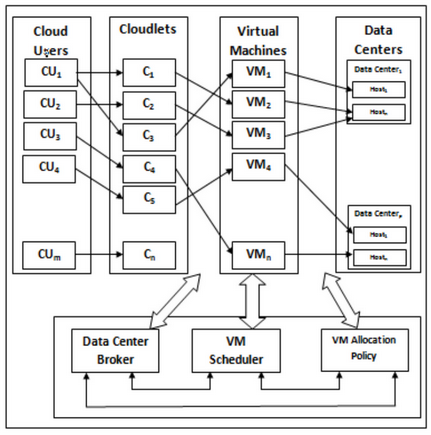
\includegraphics[scale=0.5]{media/imagenuno}
	\caption{Estilo de Trabajo de \textit{CloudSim}, Fuente: Chatterjee et al.}
	\label{fig:TrabajoCloudsim}
	
\end{figure}


Entre los componentes que proporciona dicho \textit{framework} se encuentran los siguientes:

\begin{itemize}
	\item \textit{\textbf{Cloudlet:}} Esta clase modela las aplicaciones de servicio basadas en la nube como pueden ser env\'io de contenido, redes sociales, y flujo de trabajo empresarial (\citeauthor{calheiros2011cloudsim}, \citeyear{calheiros2011cloudsim}, cap. 4).
	\item \textit{ \textbf{Datacenter:}} Esta clase modela el núcleo de los servicios en un nivel de infraestructura \textit{(hardware)} que son ofrecidos por \textit{Cloud Providers (Amazon, Azure, App Engine)}. Estos son encapsulados en un conjunto de \textit{host} que pueden ser homogéneos o heterogéneos con respecto a sus configuraciones de \textit{hardware} (memoria, n\'ucleos, capacidad, y almacenamiento) (\citeauthor{calheiros2011cloudsim}, \citeyear{calheiros2011cloudsim}, cap. 4).
	\item \textit{ \textbf{DatacenterBroker:}} Esta clase modela un \textit{broker}, el cual es responsable de mediar las negociaciones entre el \textit{SaaS} y los \textit{Cloud providers}; y dichas negociaciones son manejadas por los requerimientos \textit{QoS} (\citeauthor{calheiros2011cloudsim}, \citeyear{calheiros2011cloudsim}, cap. 4).
	\item  \textit{\textbf{Host:}} Esta clase modela los recursos f\'isicos como una computadora o un servidor de almacenamiento (\citeauthor{calheiros2011cloudsim}, \citeyear{calheiros2011cloudsim}, cap. 4).
	\item  \textit{\textbf{Vm:}} Esta clase modela una M\'aquina Virtual \textit{(VM)}, la cual es administrada y hosteada por un componente \textit{host} en la nube. Cada \textit{VM} tiene acceso a un componente que almacena las siguientes características relacionadas a una \textit{VM}: memoria accesible, procesador, tamaño de almacenamiento (\citeauthor{calheiros2011cloudsim}, \citeyear{calheiros2011cloudsim}, cap. 4).
\end{itemize}


\newpage

\subsection{Implementaci\'on de los Algoritmos}

Existen varios algoritmos para calendarizar los trabajos en el c\'omputo en la nube. La mayor ventaja de estos algoritmos es obtener el mayor rendimiento. Los principales ejemplos de algoritmos de calendarizaci\'on son: \textit{FCFS, Round Robin, Min-Min, Max-Min y algoritmos de metaheurísticas}  (\citeauthor{shimpy2014different}, \citeyear{shimpy2014different}, p. 1).



De los algoritmos mencionados anteriormente, se presentan los siguientes:


\begin{itemize}
	\item \textit{\textbf{FCFS:}} Ejecuta las tareas en orden de llegada, es decir, el primero en llegar es el primero en ser atendido.
	\item \textit{\textbf{Min-Min:}} Selecciona las tareas m\'as pequeñas para ser ejecutadas primero.
	\item  \textit{\textbf{Max-Min:}} Selecciona las tareas m\'as grandes para ser ejecutadas primero.
\end{itemize}

En un entorno de trabajo normal, la forma descrita anteriormente la podemos ver de la siguiente manera, Figura (\ref{fig:cuatro}):


\setcounter{figure}{3}
\renewcommand\thefigure{\arabic{figure}}
\begin{figure}[H]
	\centering
	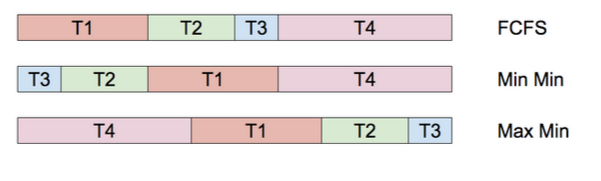
\includegraphics[scale=0.7]{media/imagendos}
	\caption{Esquema de trabajo de algoritmos de calendarizaci\'on, Fuente: Elaboraci\'on propia.}
	\label{fig:cuatro}
\end{figure}


Sin embargo en un entorno en la nube, al ser m\'ultiples m\'aquinas virtuales alojadas en distintos \textit{hosts}, que a su vez pueden formar parte de uno o m\'as \textit{datacenters}, dicho esquema tiene que ser modificado para poder adoptar un estilo de trabajo similar al proporcionado por el \textit{framework}, por lo que los resultados quedan de la distinta manera:

\newpage

\setcounter{figure}{4}
\renewcommand\thefigure{\arabic{figure}}
\begin{figure}[h!]
	\centering
	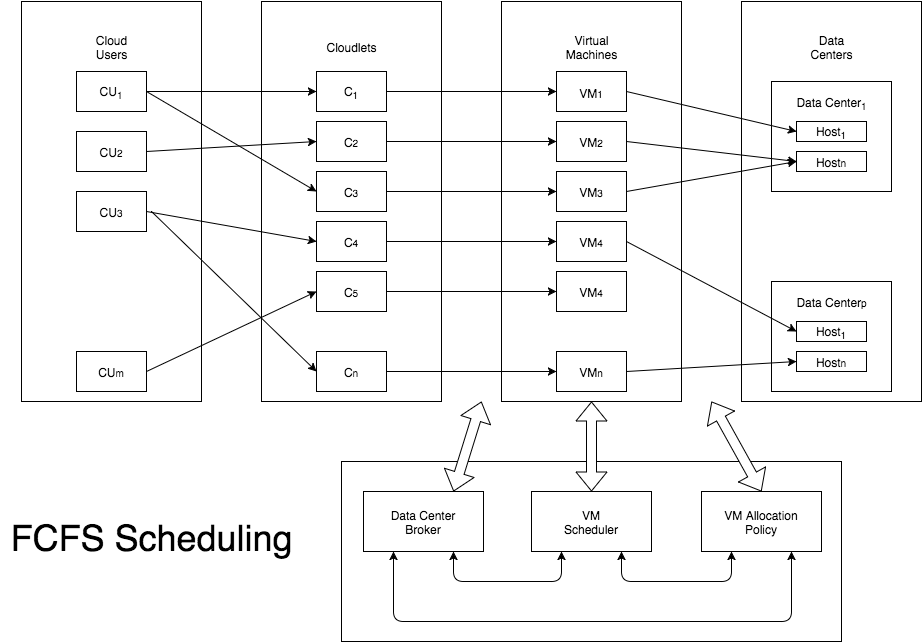
\includegraphics[scale=0.4]{media/imagentres}
	\caption{Arquitectura FCFS para un entorno en la nube. Fuente: Elaboraci\'on propia.}
	\label{fig:fcfs}
\end{figure}

Como podemos apreciar en el diagrama (Figura \ref{fig:fcfs}), podemos tener \emph{m} usuarios ejecutando \emph{n} tareas, sin embargo la asignaci\'on de m\'aquinas virtuales va dependiendo del orden de llegada de dichas tareas, y quien se encarga de repartir las tareas es el \textit{datacenterBroker}.

De manera similar tenemos los siguientes algoritmos \textit{Min-Min} (Figura \ref{fig:min}) y \textit{Max-Min} (Figura \ref{fig:max}):

\newpage

\setcounter{figure}{5}
\renewcommand\thefigure{\arabic{figure}}
\begin{figure}[h!]
	\centering
	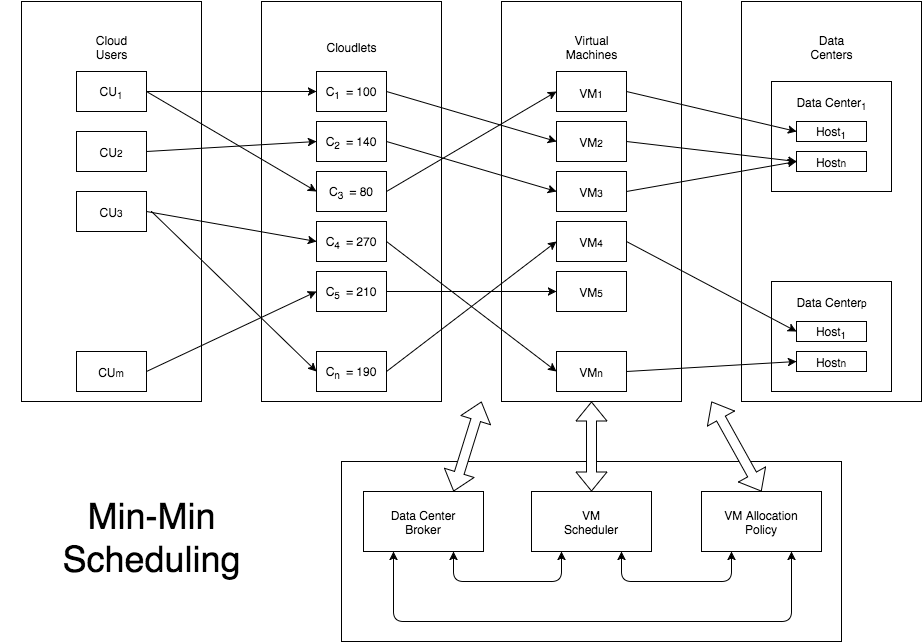
\includegraphics[scale=0.5]{media/imagencinco}
	\caption{Arquitectura de \textit{Min-Min} para un entorno en la nube. Fuente: Elaboraci\'on propia.}
	\label{fig:min}
\end{figure}

Para el algoritmo de \textit{Min-Min} (Figura \ref{fig:min}), obtenemos la lista de tareas a partir de la informaci\'on de ellas, procedemos a ordenarlas de menor a mayor tama\~no, asignando la de menor tama\~no en la primera m\'aquina virtual, la siguiente tarea, de acuerdo al tama\~no, pasa a la segunda m\'aquina y as\'i sucesivamente.

\newpage
\setcounter{figure}{6}
\renewcommand\thefigure{\arabic{figure}}
\begin{figure}[h!]
	\centering
	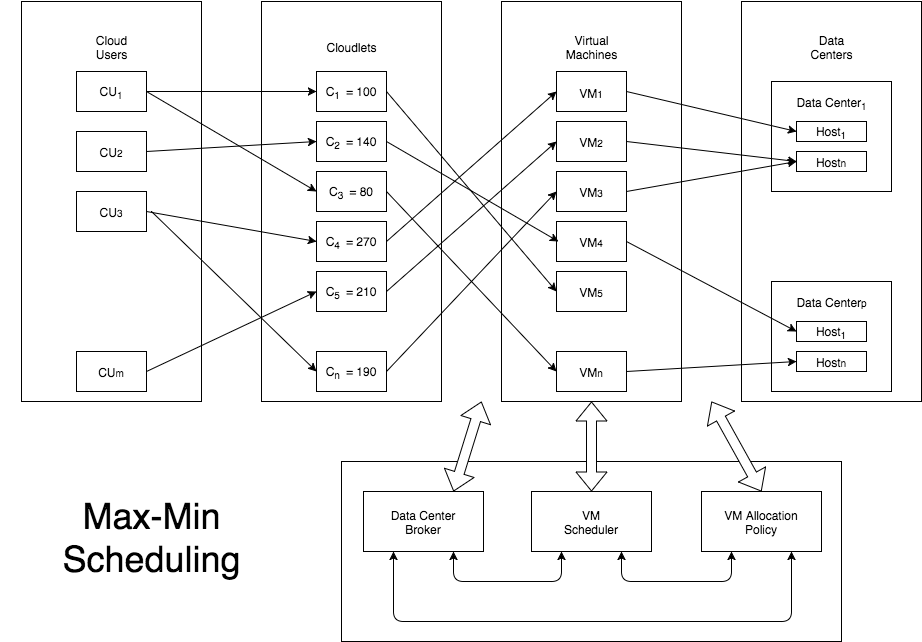
\includegraphics[scale=0.5]{media/imagencuatro}
	\caption{Arquitectura de \textit{Max-Min} para un entorno en la nube. Fuente: Elaboraci\'on propia.}
	\label{fig:max}
\end{figure}

En la figura (\ref{fig:max}) tenemos el algoritmo de \textit{Max-Min}, el cual ordena la lista de tareas de mayor a menor tama\~no antes de asignarlas a las m\'aquinas virtuales, una vez ordenada dicha lista procede a asignar la tarea m\'as grande en la primera m\'aquina, la siguiente en la segunda y as\'i sucesivamente hasta terminar la asignaci\'on de las tareas.\\



A continuaci\'on se muestran algunas capturas del c\'odigo para la implementaci\'on de los primeros algoritmos en el centro de datos:

\newpage

\subsection*{Configuración de Elementos del \textit{Datacenter} y \textit{DatacenterBrokers} para Algoritmos de Calendarización}
\addcontentsline{toc}{section}{Configuración de Elementos del Datacenter y DatacenterBrokers para Algoritmos de Calendarización}

\setcounter{figure}{7}
\renewcommand\thefigure{\arabic{figure}}
\begin{figure}[h!]
	\centering
	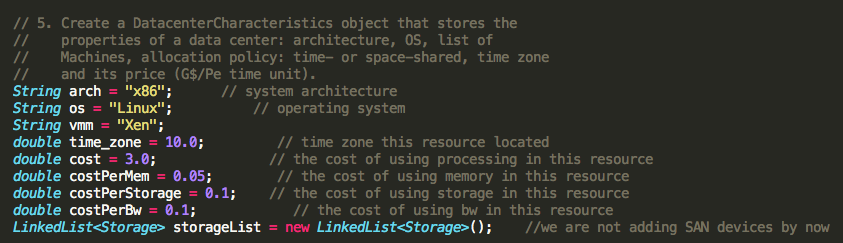
\includegraphics[scale=0.5]{media/caracteristicas_datacenter}
	\caption{Características del \textit{datacenter}. Fuente: Elaboración propia}
	\label{fig:DCar}
\end{figure}


Como primer paso,  debemos de configurar las caracter\'isticas que tendrá nuestro \textit{datacenter}, para eso tenemos que definir la arquitectura, el tipo de sistema operativo, costos de utilizaci\'on de memoria, almacenamiento y ancho de banda, entre otros (Figura \ref{fig:DCar}).


\setcounter{figure}{8}
\renewcommand\thefigure{\arabic{figure}}
\begin{figure}[h!]
	\centering
	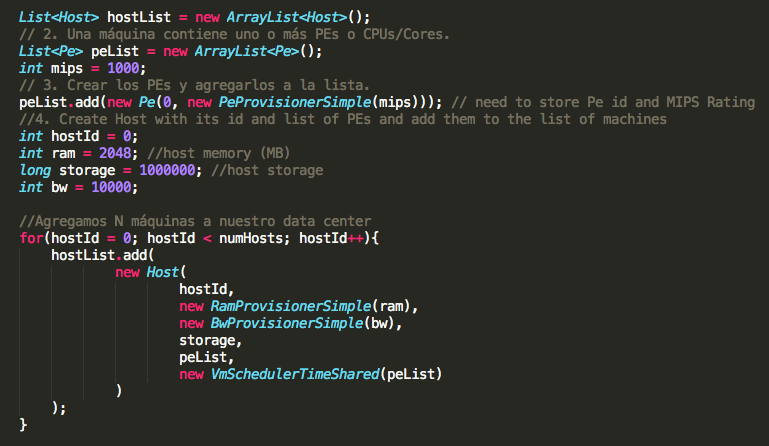
\includegraphics[scale=0.5]{media/caracteristicas_host}
	\caption{Características del \textit{Host}. Fuente: Elaboración propia}
	\label{fig:HCar}
	
\end{figure}

De igual manera tenemos que asignar las caracter\'isticas que tendr\'a cada \textit{host} dentro del \textit{datacenter} (Figura \ref{fig:HCar}), tales como el n\'umero de procesadores, n\'umero de instrucciones por segundo, memoria RAM, capacidad de almacenamiento y el ancho de banda.

\setcounter{figure}{9}
\renewcommand\thefigure{\arabic{figure}}
\begin{figure}[h!]
	\centering
	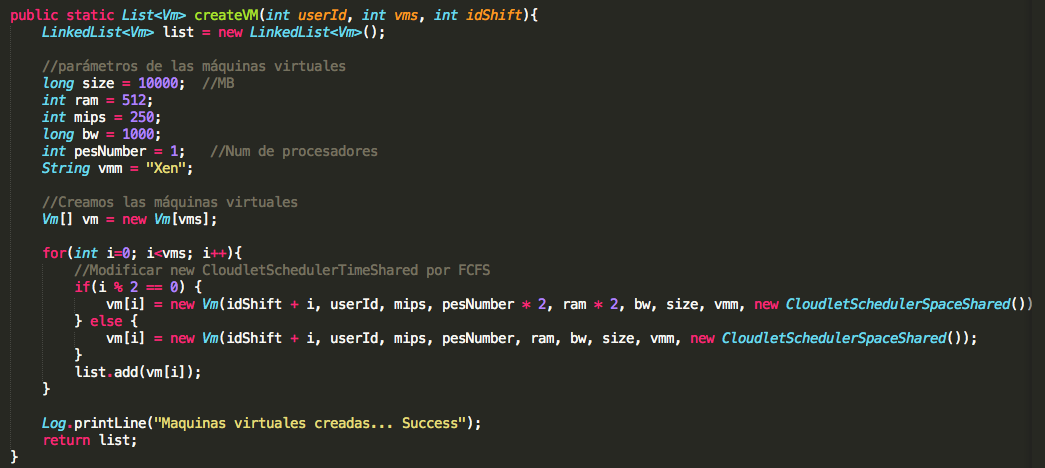
\includegraphics[scale=0.3]{media/creacion_vm}
	\caption{Características de las máquinas virtuales. Fuente: Elaboración propia}
	\label{fig:VCar}
\end{figure}


Continuando con las configuraciones, en la Figura (\ref{fig:VCar}) se muestran las caracter\'isticas utilizadas en las m\'aquinas virtuales, las cuales son: tamaño de la imagen, memoria RAM virtual, n\'umero de instrucciones por segundo, ancho de banda y el n\'umero de procesadores.


\setcounter{figure}{10}
\renewcommand\thefigure{\arabic{figure}}
\begin{figure}[h!]
	\centering
	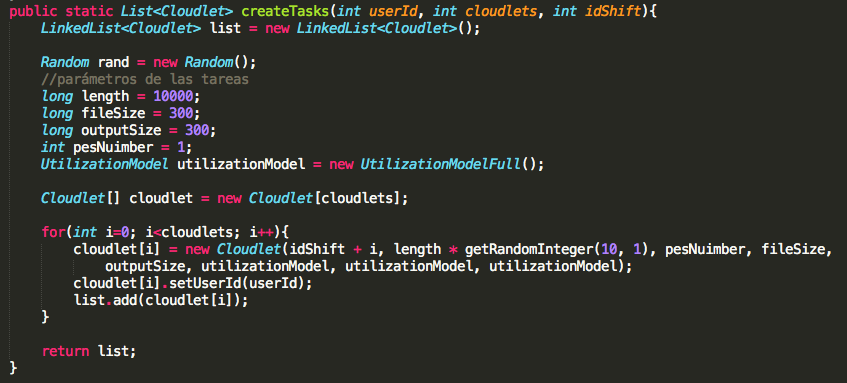
\includegraphics[scale=0.5]{media/creacion_cloudlet}
	\caption{Características de las Tareas \textit{(cloudlets)}. Fuente: Elaboración propia}
	\label{fig:TCar}
\end{figure} 




\newpage

Adem\'as de los recursos, se debe de hacer la configuraci\'on de las tareas a simular (Figura \ref{fig:TCar}), teniendo como par\'ametros el tamaño de la tarea, tamaño de entrada y de salida, as\'i como el número de procesadores que ocupar\'a la tarea, esto \'ultimo refleja la complejidad de la tarea.

\subsection*{\textit{DatacenterBrokers} para Algoritmos de Calendarización}
\addcontentsline{toc}{section}{DatacenterBrokers para Algoritmos de Calendarización}

Partiendo del Esquema que se muestra en la figura (\ref{fig:TrabajoCloudsim}), el trabajo presentado se lleva a cabo en la parte de Tareas (\textit{cloudlets}) y M\'aquinas Virtuales (\textit{Virtual Machines}) ya que se pretende mejorar un algoritmo de calendarizaci\'on de tareas.
Para ello seg\'un muestra el diagrama, el encargado de asignar cada tarea en una m\'aquina virtual es el \textit{datacenter broker}, el cual toma la lista de tareas as\'i como la lista de m\'aquinas virtuales, y de acuerdo a alg\'un algoritmo realiza la asignaci\'on de cada una de las tareas en las distintas m\'aquinas virtuales disponibles.

\newpage

\setcounter{figure}{11}
\renewcommand\thefigure{\arabic{figure}}
\begin{figure}[h!]
	\centering
	\includegraphics[scale=0.5]{media/FCFS_broker}
	\caption{\textit{FCFS Broker}. Fuente: Elaboración propia}
	\label{fig:fcfsBroker}
\end{figure}

La Figura (\ref{fig:fcfsBroker}) muestra el algoritmo de \textit{FCFS}, recorre la lista de tareas y la asigna en la m\'aquina virtual correspondiente, calculando la tarea actual $i$ en la m\'aquina virtual \textbf{$i\%reqVms$} donde \textbf{$reqVms$} es el n\'umero de m\'aquinas virtuales.

\setcounter{figure}{12}
\renewcommand\thefigure{\arabic{figure}}
\begin{figure}[h!]
	\centering
	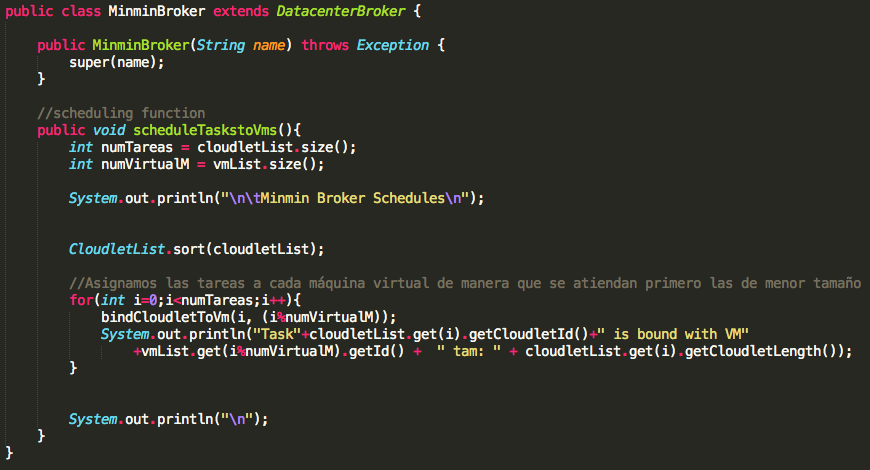
\includegraphics[scale=0.5]{media/minmin_broker}
	\caption{\textit{Min-Min Broker}. Fuente: Elaboración propia}
	\label{fig:minminBroker}
\end{figure}

\newpage

En la Figura (\ref{fig:minminBroker}) tenemos la implementaci\'on del algoritmo \textit{Min-Min} en el cual podemos apreciar el ordenamiento de la lista antes de pasar a  la asignaci\'on de las m\'aquinas virtuales.

\newpage
\setcounter{figure}{13}
\renewcommand\thefigure{\arabic{figure}}
\begin{figure}[h!]
	\centering
	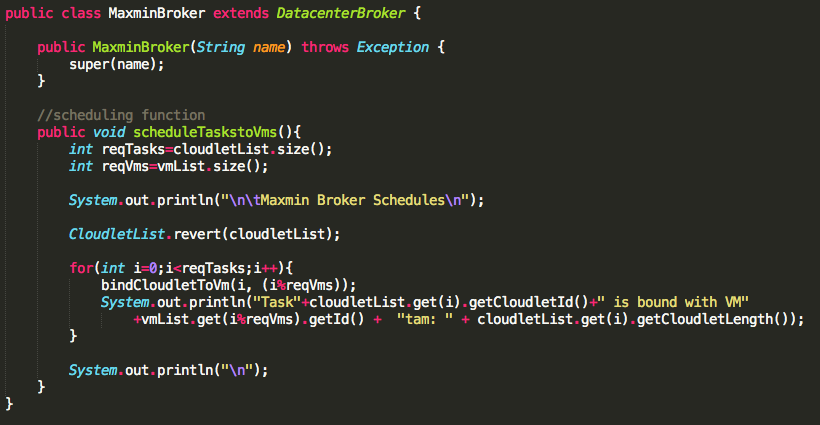
\includegraphics[scale=0.5]{media/maxmin_broker}
	\caption{\textit{Max-min Broker}. Fuente: Elaboración propia}
	\label{fig:maxminBroker}
\end{figure}

En la Figura (\ref{fig:maxminBroker}) observamos la implementaci\'on del algoritmo de \textit{Max-Min} el cual hace un ordenamiento de mayor a menor, v\'ease la funci\'on \textbf{\textit{revert}} utilizada, la cual se explicar\'a m\'as adelante.

\newpage


%\setcounter{figure}{14}
\renewcommand\thefigure{\arabic{figure}}
\begin{figure}[h!]
	\centering
	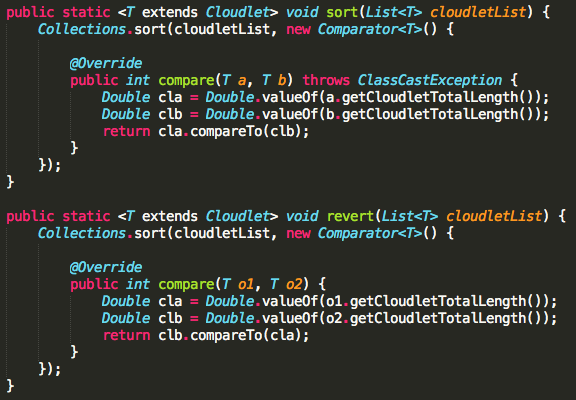
\includegraphics[scale=0.5]{media/ordenamientos}
	\caption{\textit{Algoritmos de ordenamientos}. Fuente: Elaboración propia}
	\label{fig:sortRevert}
\end{figure}

En la Figura (\ref{fig:sortRevert}) tenemos la implementaci\'on de los m\'etodos de ordenamiento utilizados, el \textbf{sort} utilizado para ordenar las tareas de menor a mayor de acuerdo al tamaño y el \textbf{revert} de forma inversa.

%ver la seccion anexo